\documentclass{article}
\usepackage[utf8]{inputenc}
\usepackage[spanish]{babel}
\usepackage{amsmath}
\usepackage{multicol}
\usepackage{graphicx}
\usepackage{float}
\usepackage{geometry}
\usepackage{listings}
\usepackage{enumitem}

\title{Report of the model SIR}
\author{PropEnfermedades APP}
\date{}
\geometry{letterpaper, top=2.54cm, bottom=2.54cm, left=3cm, right=3cm}    
\setlength{\parindent}{0cm}
\setlength{\parskip}{0.2em}

\begin{document}
\maketitle
\section{Model}
Next we show the model used in the simulation.
\subsection*{Description}
SIR model, which represents the spread of an infectious disease in a population.
\subsection*{Equations}
\begin{equation}
\begin{split}
S' = -b * S * I \\ I' = b * S * I - k * I \\ R' = k * I
\end{split}
\end{equation}
\subsection*{Parameters}
\begin{itemize}
\item $b = 2$. 
\item $k = 0.6$. 
\end{itemize}
\subsection*{Initial values}
The initial values used in the simulation are (The values are normalized respect to 7900000 that is the total population):
\begin{itemize}
\item $S_0 = 0.999999$. 
\item $I_0 = 1.26582e-06$. 
\item $R_0 = 0$. 
\item $t_0 = 0$. 
\item $t_f = 100$. 
\item $dt = 0.5$. 
\end{itemize}
\section*{Results}
The maximum infected population is 2.80068e+06 is reached on day 10.5.
Next we show the results of the simulation using the model SIR with the parameters and initial values shown above.
\begin{figure}[H]
\centering
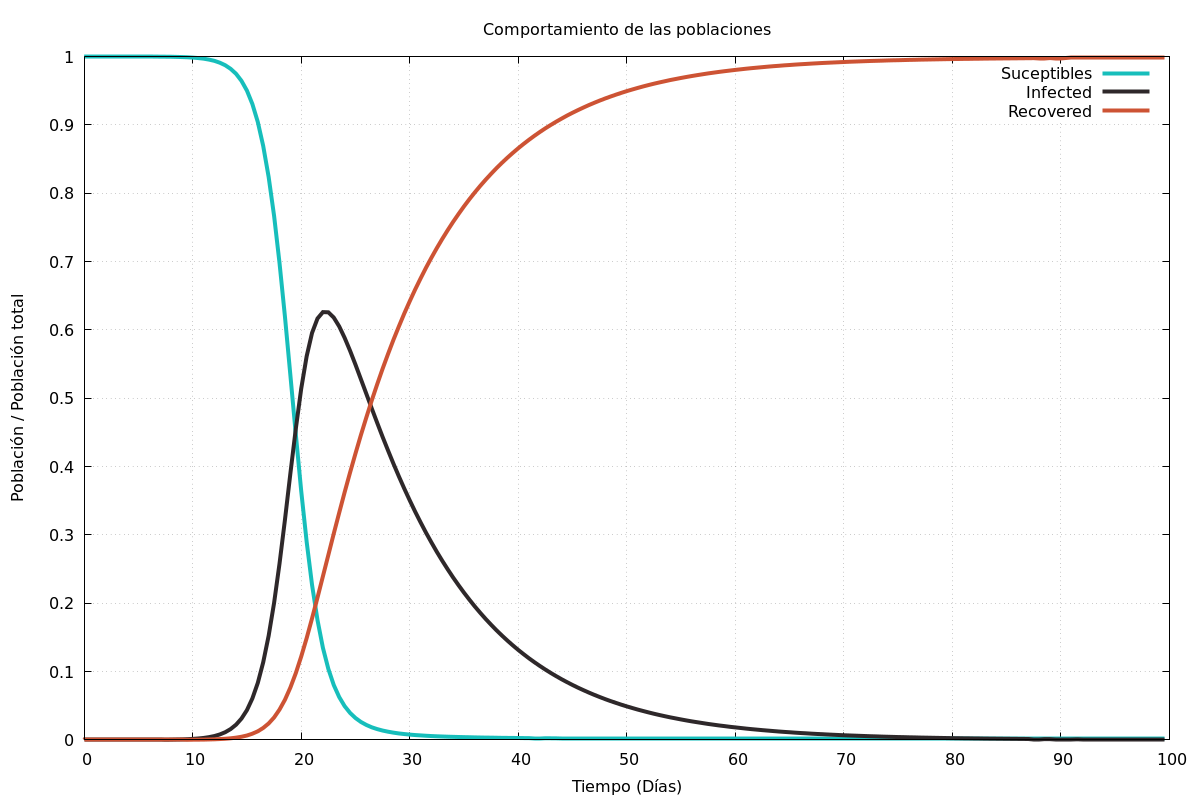
\includegraphics[width=0.8\textwidth]{./data/Prueba2/graph-SIR.png}
\caption{Graph of the model SIR}
\end{figure}
\begin{figure}[H]
\centering
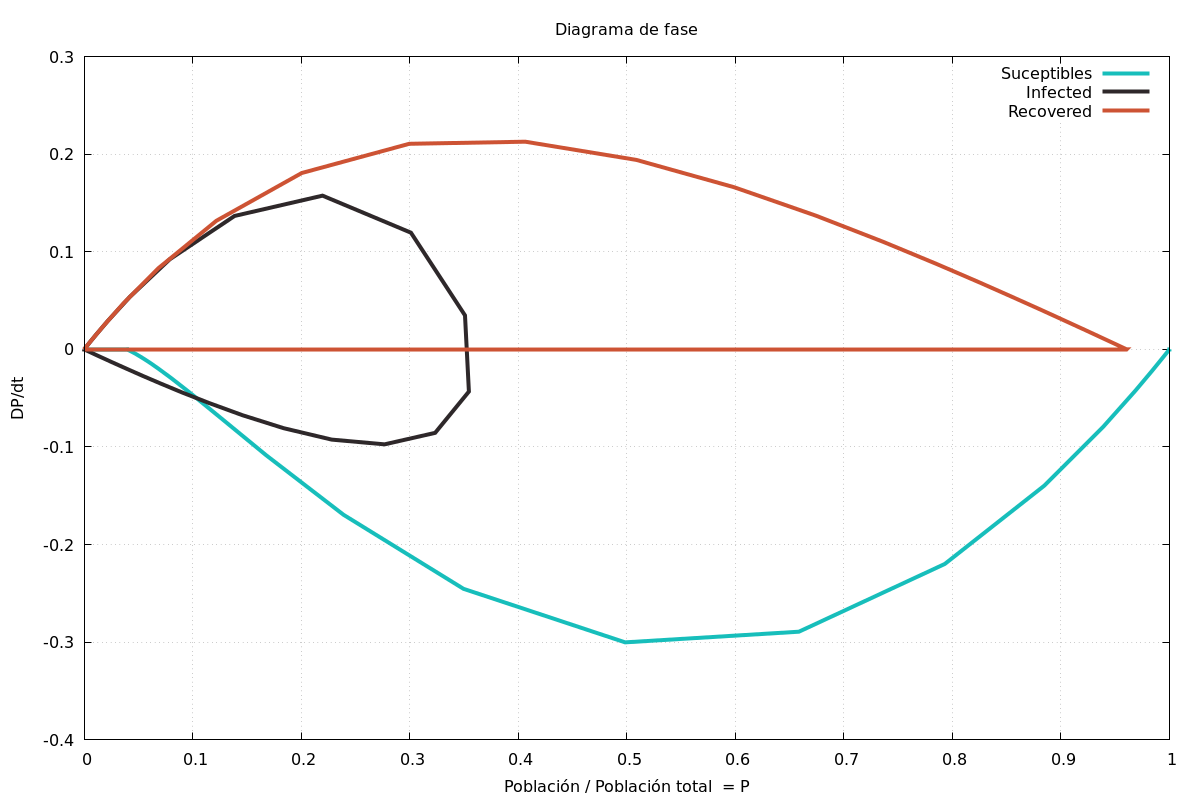
\includegraphics[width=0.8\textwidth]{./data/Prueba2/phase-SIR.png}
\caption{Phase portrait of the model SIR}
\end{figure}
\end{document}
